\section{Experiments}
\label{sec:experiments}

% Description of your testbed;
% List of questions your experiments are designed to answer.
% Details of the experiments; observations.

\subsection{Adding Noise into Logistic Regression}
In these experiments, we intorduce noise into gradient descent component
of Logistic Regression.
To be more specific, in a noise-free Logistic Regression model, weights
are updated in the following way:
\[
W_{new} = W_{old} - \lr \nabla_{W_{old}} \cost(W)
\]
In a noise-added Logistic Regression model, weights are updated as:
\[
W_{new}=W_{old}-\lr \left(\mask \cdot \nabla_{W_{old}}\cost(W) \right)
\]
or
\[
W_{new} = W_{old} - \mask_{Gau} \cdot \nabla_{W_{old}} \cost(W)
\]
where learning rate is a scalar and mask is a vector that has the same dimension as $W_t$.

We generate mask as a random vector from Binomial distribution
$Bin(1,0.5)$, Gaussian distribution $\mathcal{N}(\lr, 2 \cdot \lr)$,
Rayleigh Distribution and Gamma Distribution $Gamma(1)$, respectively.
Figure~\ref{logistic} shows test error rate using noise-free and
noise-added Logistic Regression.
\begin{figure}[!htbp]
\centering
\label{logistic}
\caption{Logistic Regression with Noise}
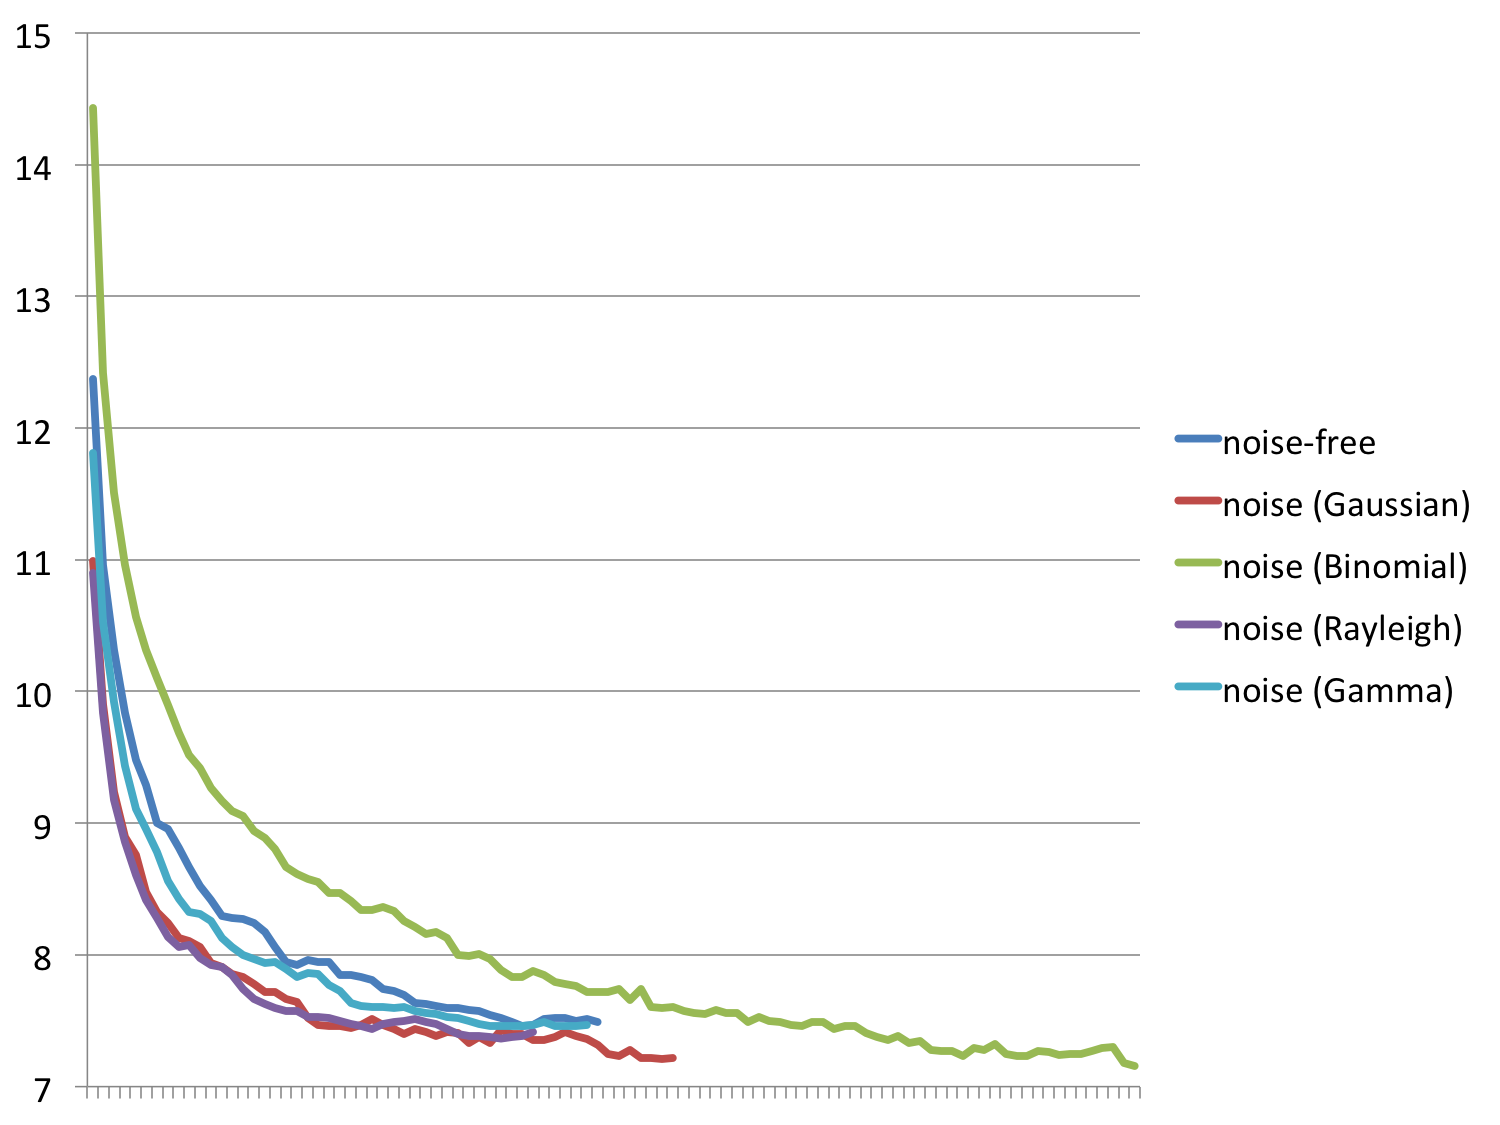
\includegraphics[width=\textwidth]{f-figs/logistic.png}
\end{figure}

% explain the figure

\subsection{Adding Noise into Multi-layer Logistic Regression}
In these experiments, we introduce noise into

\subsection{Adding Noise into Convolutionary Neural Network}


